\item A smooth rubber cord of length $l$ whose coefficient of elasticity is $k$ is suspended by one end from the point $O$ (Fig. 1.33). The other end is fitted with a catch $B$. A small sleeve $A$ of mass $m$ starts falling from the point $O$. Neglecting the masses of the thread and the catch, find the maximum elongation of the cord.
    \begin{center}
        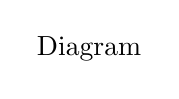
\begin{tikzpicture}
            \node at (0, 0) {Diagram};
        \end{tikzpicture}
    \end{center}\begin{solution}
    \begin{align*}
        \intertext{Suppose that $\Delta l$ is the elongation of the rubber cord. Then, from energy conservation}
        \Delta U_{gr} + \Delta U_{el} &= 0 \quad \text{(as $\Delta T = 0$)} \tag{1.139.1}\\
        \intertext{or}
        -mg \left(l + \Delta l \right) + \dfrac{1}{2} \kappa \Delta l^2 &= 0 \tag{1.139.2}\\
        \intertext{or}
        \dfrac{1}{2} \kappa \Delta l^2 - mg \Delta l - mgl &= 0 \tag{1.139.3}\\
        \intertext{or}
        \Delta l &= \dfrac{mg \pm \sqrt{(mg)^2 + 4 \times \dfrac{\kappa}{2} mgl}}{2 \times \dfrac{\kappa}{2}} = \dfrac{mg}{\kappa} \left[ 1 + \sqrt{1 \pm \dfrac{2 \kappa l}{mg}} \right] \tag{1.139.4} \\
        \intertext{Since the value of $\sqrt{1 + \dfrac{2 \kappa l}{mg}}$ is certainly greater than $1$, hence negative sign is avoided.}
        \intertext{So,}
        \Delta l &= \dfrac{mg}{\kappa} \left( 1 + \sqrt{1 + \dfrac{2 \kappa l}{mg}} \right)
    \end{align*}
\end{solution}